%\VignetteIndexEntry{RandVar}
%\VignetteDepends{distr,distrEx}
%\VignetteKeywords{random variable, S4 classes, S4 methods}
%\VignettePackage{RandVar}
%
\documentclass[11pt]{article}
\usepackage{geometry}\usepackage{color}
\usepackage{ifpdf}
\definecolor{darkblue}{rgb}{0.0,0.0,0.75}
\usepackage[%
baseurl={http://www.stamats.de},%
pdftitle={RandVar: Implementation of random variables by means of S4 classes and methods},%
pdfauthor={Matthias Kohl},%
pdfsubject={RandVar},%
pdfkeywords={random variable, S4 classes, S4 methods},%
pagebackref,bookmarks,colorlinks,linkcolor=darkblue,citecolor=darkblue,%
pagecolor=darkblue,raiselinks,plainpages,pdftex]{hyperref}
%
\markboth{\sl Packages ``{\tt RandVar}''}{\sl Packages ``{\tt RandVar}''}
%
% -------------------------------------------------------------------------------
\newcommand{\code}[1]{{\tt #1}}
\newcommand{\pkg}[1]{{\tt "#1"}}
\newcommand{\pkgversion}{{\tt 2.0}}
\newcommand{\pkgExversion}{{\tt 0.6.2}}
% -------------------------------------------------------------------------------
%
% -------------------------------------------------------------------------------
\usepackage{/home/btm722/RTOP/R-2-7-branch/share/texmf/Sweave}
\begin{document}
% -------------------------------------------------------------------------------
\title{RandVar: Implementation of random variables by means
    of {\tt S4} classes and methods}
\author{Matthias Kohl\\
e-Mail: {\tt matthias.kohl@stamats.de}\\
}
\maketitle
% -------------------------------------------------------------------------------
\begin{abstract}
% -------------------------------------------------------------------------------
In this package we implement random variables by means of {\tt S4} classes
and methods. This vignette corresponds to Appendix D.2 in Kohl~(2005)~\cite{MK:05}.
% -------------------------------------------------------------------------------
\end{abstract}
% -------------------------------------------------------------------------------
\tableofcontents
% -------------------------------------------------------------------------------
\clearpage
% -----------------------------------------------------------------------
\section{{\tt S4} Classes}
% -----------------------------------------------------------------------
The {\tt S4} class {\tt RandVariable} (cf.\ Figure~\ref{ap.Rpack.RandVar.dia1})
has the slots {\tt Map}, {\tt Domain} and {\tt Range} where {\tt Map}
contains a list of functions which are measurable maps from {\tt Domain}
to {\tt Range}. The elements contained in the list {\tt Map} must be functions in 
one argument named {\tt x}. We do not allow further parameters for these 
functions as this would lead to inconsistent objects. Strictly speaking, an object of 
class {\tt RandVariable} would represent not only one random variable but a whole 
set of random variables depending on these parameters.
% -----------------------------------------------------------------------
\par
The slots {\tt Domain} and {\tt Range} are filled with an object of
class {\tt OptionalrSpace}; i.e., they contain {\tt NULL} or an object of class 
{\tt rSpace} (see package {\tt distr}~\cite{distr}). In case of
{\tt EuclRandVariable} and {\tt RealRandVariable} the slot {\tt Range} is filled 
with an object of class {\tt Euclideanspace} and {\tt Reals}, respectively. The 
class {\tt EuclRandMatrix} additionally has the slot {\tt Dim} which is a vector 
of integers and contains the dimensions of the Euclidean random matrix.
% -----------------------------------------------------------------------
\par
Using these {\tt S4} classes there are two possibilities to implement a ${\rm R}^k$
valued random variable. First, we could define a {\tt EuclRandVariable}
whose slot {\tt Map} contains a list with one function which maps to ${\rm R}^k$;
i.e., the slot {\tt Range} is a $k$-dimensional Euclidean space. Second, we could
define a {\tt EuclRandVariable} whose slot {\tt Map} contains a list with $n$
functions (projections) which map to ${\rm R}^m$ where $k = m*n$. Now, the slot
{\tt Range} is an $m$-dimensional Euclidean space.
Since it is sometimes convenient to regard a ${\rm R}^k$ valued random variable
as measurable map consisting of ${\rm R}^{k_i}$ valued maps where $\sum k_i = k$,
we introduce a further class called {\tt EuclRandVarList}.
With this class we can now define ${\rm R}^k$ valued random variables as a list
of ${\rm R}^{k_i}$ valued random variables with compatible domains. More precisely,
the elements of a {\tt EuclRandVarList} may even have very different ranges
(not necessarily Euclidean spaces) they only need to have compatible
domains which is checked via the generic function {\tt compatibleDomains}.
% -----------------------------------------------------------------------
\begin{figure}[!ht]
\begin{center}
  \ifpdf
    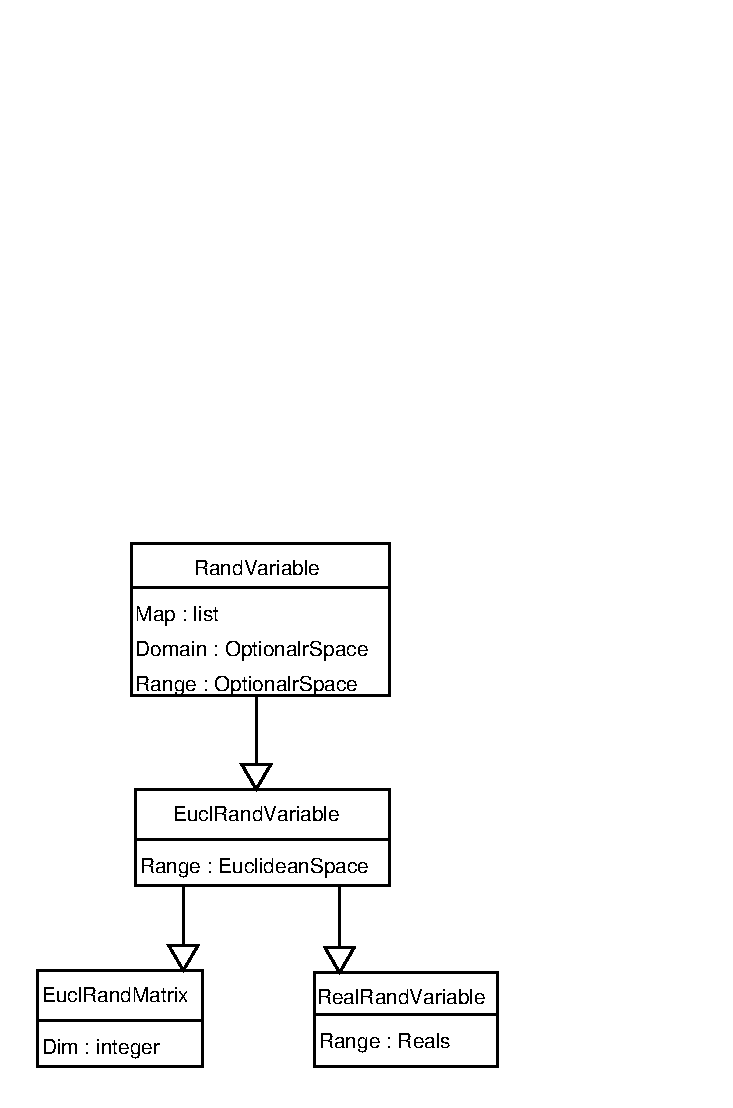
\includegraphics[scale=1.0, viewport = 14 15 244 275]{RandVariable.pdf}
  \else
    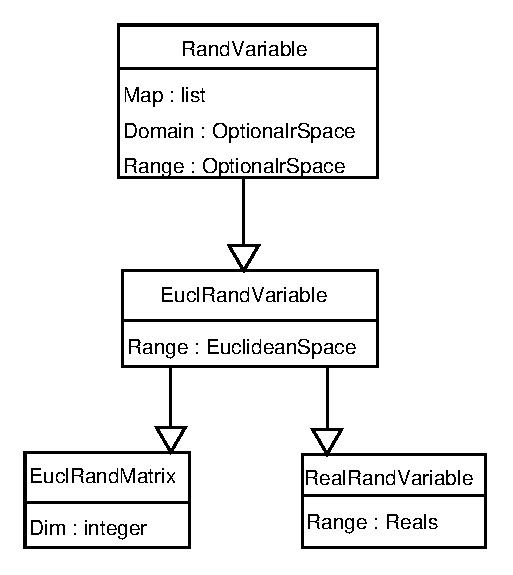
\includegraphics[scale=1.0]{RandVariable.eps}
  \fi
  \caption[Class {\tt RandVariable} and Subclasses]{Class
    {\tt RandVariable} and subclasses.}
  \label{ap.Rpack.RandVar.dia1}
\end{center}
\end{figure}
% -----------------------------------------------------------------------
\newpage
\section{Functions and Methods}
% -----------------------------------------------------------------------
As in case of package {\tt distrEx}~\cite{distr}, we follow the advices of 
Section~7.3 of \cite{Cham:98} and \cite{Gent:03}. That is, we introduce 
generating functions as well as accessor and replacement functions. A short
description of the implemented generating functions is given in
Table~\ref{ap.Rpack.RandVar.tab.gen}.
% -----------------------------------------------------------------------
\begin{table}[!ht]
\begin{center}
\begin{tabular}{p{4cm}|p{7.5cm}}
  \textbf{Generating Function} & \textbf{Description} \\ \hline\hline
  {\tt EuclRandMatrix} & Generates an object of class {\tt EuclRandMatrix}\\ \hline
  {\tt EuclRandVariable} & Generates an object of class {\tt EuclRandVariable}\\ \hline
  {\tt EuclRandVarList}   & Generates an object of class {\tt EuclRandVarList}\\ \hline
  {\tt RandVariable} & Generates an object of class {\tt RandVariable}\\ \hline
  {\tt RealRandVariable} & Generates an object of class {\tt RealRandVariable}
\end{tabular}
\caption[Generating Functions of Package {\tt RandVar}]{Generating
functions of package {\tt RandVar}.}\label{ap.Rpack.RandVar.tab.gen}%
\end{center}
\end{table}
% -----------------------------------------------------------------------
\par\noindent
While there are accessor functions for all slots of the newly defined
{\tt S4} classes, replacement functions are only implemented for those
slots a user should modify.
% -----------------------------------------------------------------------
\par
Our next goal was that one can use these classes of random variables like
ordinary numeric vectors or matrices. Hence, we overloaded the {\tt S4}
group generic functions {\tt Arith} and {\tt Math} as well as matrix
multiplication {\tt \%*\%}. For the matrix multiplication of {\tt EuclRandVarList}s 
we additionally introduced the operator {\tt \%m\%}.
Now, if we have random variables {\tt X} and {\tt Y}, a numerical
vector {\tt v} and a numerical matrix {\tt M} (with compatible dimensions)
we can for instance generate
\begin{Schunk}
\begin{Sinput}
> library(RandVar)
> (X <- RealRandVariable(Map = list(function(x) {
+     x
+ }, function(x) {
+     x^2
+ }), Domain = Reals(), Range = Reals()))
\end{Sinput}
\begin{Soutput}
An object of class “RealRandVariable” 
length of Map:	 2 
Domain:	Real Space with dimension 1 
Range:	Real Space with dimension 1 
\end{Soutput}
\begin{Sinput}
> Map(X)
\end{Sinput}
\begin{Soutput}
[[1]]
function (x) 
{
    x
}

[[2]]
function (x) 
{
    x^2
}
\end{Soutput}
\begin{Sinput}
> evalRandVar(X, 2)
\end{Sinput}
\begin{Soutput}
     [,1]
[1,]    2
[2,]    4
\end{Soutput}
\begin{Sinput}
> evalRandVar(X, as.matrix(seq(2, 10, 2)))
\end{Sinput}
\begin{Soutput}
, , 1

     [,1] [,2] [,3] [,4] [,5]
[1,]    2    4    6    8   10
[2,]    4   16   36   64  100
\end{Soutput}
\begin{Sinput}
> R1 <- exp(X - 1)
> Map(R1)
\end{Sinput}
\begin{Soutput}
[[1]]
function (x) 
{
    f1 <- function (x) 
    {
        f1 <- function (x) 
        {
            x
        }
        f1(x) - 1
    }
    exp(f1(x))
}
<environment: 0x8cd175c>

[[2]]
function (x) 
{
    f1 <- function (x) 
    {
        f1 <- function (x) 
        {
            x^2
        }
        f1(x) - 1
    }
    exp(f1(x))
}
<environment: 0x8cd175c>
\end{Soutput}
\begin{Sinput}
> R2 <- exp(X - 1:2)
> Map(R2)
\end{Sinput}
\begin{Soutput}
[[1]]
function (x) 
{
    f1 <- function (x) 
    {
        f1 <- function (x) 
        {
            x
        }
        f1(x) - 1L
    }
    exp(f1(x))
}
<environment: 0x90d97e4>

[[2]]
function (x) 
{
    f1 <- function (x) 
    {
        f1 <- function (x) 
        {
            x^2
        }
        f1(x) - 2L
    }
    exp(f1(x))
}
<environment: 0x90d97e4>
\end{Soutput}
\begin{Sinput}
> (Y <- RealRandVariable(Map = list(function(x) {
+     sin(x)
+ }, function(x) {
+     cos(x)
+ }), Domain = Reals(), Range = Reals()))
\end{Sinput}
\begin{Soutput}
An object of class “RealRandVariable” 
length of Map:	 2 
Domain:	Real Space with dimension 1 
Range:	Real Space with dimension 1 
\end{Soutput}
\begin{Sinput}
> Map(Y)
\end{Sinput}
\begin{Soutput}
[[1]]
function (x) 
{
    sin(x)
}

[[2]]
function (x) 
{
    cos(x)
}
\end{Soutput}
\begin{Sinput}
> R3 <- X %*% Y
> dimension(R3)
\end{Sinput}
\begin{Soutput}
[1] 1
\end{Soutput}
\begin{Sinput}
> 2 * sin(2) + 2^2 * cos(2)
\end{Sinput}
\begin{Soutput}
[1] 0.1540075
\end{Soutput}
\begin{Sinput}
> (R4 <- X %*% t(Y))
\end{Sinput}
\begin{Soutput}
An object of class “EuclRandMatrix” 
Dim of Map:	 2 2 
Domain:	Real Space with dimension 1 
Range:	Euclidean Space with dimension 1 
\end{Soutput}
\begin{Sinput}
> dimension(R4)
\end{Sinput}
\begin{Soutput}
[1] 4
\end{Soutput}
\begin{Sinput}
> (M <- matrix(c(2 * sin(2), 2^2 * sin(2), 2 * cos(2), 2^2 * cos(2)), 
+     ncol = 2))
\end{Sinput}
\begin{Soutput}
         [,1]       [,2]
[1,] 1.818595 -0.8322937
[2,] 3.637190 -1.6645873
\end{Soutput}
\begin{Sinput}
> (R5 <- M %*% R4)
\end{Sinput}
\begin{Soutput}
An object of class “EuclRandMatrix” 
Dim of Map:	 2 2 
Domain:	Real Space with dimension 1 
Range:	Real Space with dimension 1 
\end{Soutput}
\end{Schunk}
We also implemented {\tt S4} methods for the generic function {\tt E} of 
package {\tt distrEx}~\cite{distr}. That is, given some distribution {\tt D}, 
respectively some conditional distribution {\tt CD} and some random variable {\tt X}
we can compute the (conditional) expectation of {\tt X} under {\tt D}, respectively 
{\tt CD} simply by
\begin{Schunk}
\begin{Sinput}
> D <- Norm()
> E(object = D, fun = X)
\end{Sinput}
\begin{Soutput}
[1] 2.587378e-16 9.999942e-01
\end{Soutput}
\begin{Sinput}
> E(D)
\end{Sinput}
\begin{Soutput}
[1] 0
\end{Soutput}
\begin{Sinput}
> var(D)
\end{Sinput}
\begin{Soutput}
[1] 1
\end{Soutput}
\begin{Sinput}
> (CD <- LMCondDistribution(theta = 1))
\end{Sinput}
\begin{Soutput}
Distribution object of class: AbscontCondDistribution
theta :  1 
intercept :  0 
scale :  1 
## cond:
name:	conditioning by an Euclidean space
Range:	Euclidean Space with dimension 1
\end{Soutput}
\begin{Sinput}
> E(object = CD, fun = X, cond = 2)
\end{Sinput}
\begin{Soutput}
[1] 2.000000 4.999993
\end{Soutput}
\begin{Sinput}
> E(Norm(mean = 2))
\end{Sinput}
\begin{Soutput}
[1] 2
\end{Soutput}
\begin{Sinput}
> E(Norm(mean = 2), fun = function(x) {
+     x^2
+ })
\end{Sinput}
\begin{Soutput}
[1] 4.999993
\end{Soutput}
\end{Schunk}
for some given condition {\tt cond}.
% -----------------------------------------------------------------------
\par
In addition, we define methods for the generic function {\tt show} for the classes
{\tt RandVariable}, {\tt EuclRandMatrix} and {\tt EuclRandVarList}. There are 
also methods for the generic functions {\tt dimension} (see package 
{\tt distr}~\cite{distr}), {\tt length}, {\tt ncol}, {\tt nrow}, {\tt t} and 
{\tt [} (cf.\ package {\tt base}). For more details we refer to the corresponding 
help pages.
% -----------------------------------------------------------------------
\par
Finally, we introduce several new generic functions. A brief description
of these functions is given in Table~\ref{ap.Rpack.RandVar.tab}.
% -----------------------------------------------------------------------
\begin{table}[!ht]
\begin{center}
\begin{tabular}{p{3.5cm}|p{8cm}}
  \textbf{Generic Function} & \textbf{Description} \\ \hline\hline
  \texttt{\%m\%} & matrix multiplication for {\tt EuclRandVarList}s \\ \hline
  \texttt{compatibleDomains} & test if the domains of two random variables
                     are compatible \\ \hline
  \texttt{evalRandVar} & evaluation of random variables\\ \hline
  \texttt{imageDistr} & image distribution of some distribution under some
               random variable \\ \hline
  \texttt{numberOfMaps} & number of functions contained in the slots {\tt Map}
                 of the members of a {\tt EuclRandVarList}
\end{tabular}
\caption[New Generic Functions of Package {\tt RandVar}]
{New generic functions of package {\tt RandVar} (without accessor
and replacement functions).}\label{ap.Rpack.RandVar.tab}%
\end{center}
\end{table}
% -----------------------------------------------------------------------
\par\noindent
For more details about the full functionality of package {\tt RandVar}
we refer to the source code and the corresponding help pages, respectively.
% -----------------------------------------------------------------------
\section{Odds and Ends}
% -----------------------------------------------------------------------
The main issue is to reduce the computation time for methods using
objects of class {\tt RandVariable} and its subclasses as these classes
play an important role in the computation of optimally robust
estimators; confer Kohl~(2005)~\cite{MK:05}.
In particular, we are looking for ways to increase the computation speed
of {\tt evalRandVar} and {\tt E}.
%-------------------------------------------------------------------------------
\begin{thebibliography}{8}

\bibitem{Cham:98}
Chambers J.M. 
\newblock {\em {Programming with data. A guide to the S language}\/}.
\newblock {Springer}.
\newblock http://cm.bell-labs.com/stat/Sbook/index.html

\bibitem{Gent:03}
Gentleman R.
\newblock {\em Object Orientated Programming. Slides of a Short Course held in Auckland\/}.
\newblock http://www.stat.auckland.ac.nz/S-Workshop/Gentleman/Methods.pdf

\bibitem{MK:05}
Kohl M. 
\newblock {\em Numerical Contributions to the Asymptotic Theory of Robustness\/}. 
\newblock {Dissertation}, Universit\"at Bayreuth. 
\newblock See also http://stamats.de/ThesisMKohl.pdf

\bibitem{distr}
Ruckdeschel P., Kohl M., Stabla T., and Camphausen F. 
\newblock {S4 Classes for Distributions.} 
\newblock {\em R-News\/}, {\bf 6}(2): 10--13.
\newblock http://CRAN.R-project.org/doc/Rnews/Rnews\_2006-2.pdf
\newblock See also {http://www.uni-bayreuth.de/departments/math/org/mathe7/RUCKDESCHEL/pubs/distr.pdf}

\end{thebibliography}
% -------------------------------------------------------------------------------
\end{document}
% -------------------------------------------------------------------------------
